% 第4章第1节：向量的表示（坐标向量、相等、零向量与标准坐标向量）、向量的运算（加法与数乘、线性组合、内积、长度与距离、范数）、向量运算的性质（加法与数乘的性质、内积的性质、范数的性质）。夹角与Cauchy--Schwarz不等式见第5章内积空间一节。

\section{向量}
\label{sec:ls-vectors}
\label{sec:ls-objects}
\label{sec:linear-algebra-objects}
\label{sec:linear-algebra-space-representations}
\label{sec:prelim-vectors-matrices}

三次观测的输入与输出各是一串数；两个模型各给出一串预测，需要合并或比较；预测减去观测又是一串误差，需要判断它有多大。这些问题处理的都是按固定次序排列的一串实数，也就是向量。本节先规定向量怎样书写、何时相等；再定义向量之间的运算，回答怎样把几串数合并成一串、怎样把两串数配成一个数、怎样用一个数衡量一串数的大小；最后核对加法与数乘的基本规则。内积和范数的一般性质集中在第~\ref{chap:normed-inner-product-spaces}章讨论。

\subsection{向量的表示}
\label{sec:ls-vector-representation}
\label{sec:prelim-vector-records}

用一串数记录数据之前，须先说清这串数怎样排列、每个位置记录什么、两串数何时算作相同。

\paragraph{坐标向量}
第~\ref{sec:sets-power-sets-products}节把$\mathbb R^d$定义为全部有序$d$元实数组的集合。把其中一个元素的$d$个实数按原有次序竖排成一列，得到实坐标向量（real coordinate vector）：
\[
 \bm u=\begin{pmatrix}u_1\\\vdots\\u_d\end{pmatrix}\in\mathbb R^d,
\]
其中$u_j$是第$j$个坐标，$d$是维数。定位向量中的一个数只需要一个索引$j$。

本书默认使用这样的列向量；把同样的数横排成一行，称为行向量。上标$\top$表示\term{转置}（transpose），它把行向量改写成列向量，也把列向量改写成行向量。因此$(u_1,\ldots,u_d)^\top$就是上面的列向量，正文中常用这种写法节省篇幅。

用向量记录数据时，每个位置的含义须预先固定。例如三次观测的（输入，输出）依次为$(1,0)$、$(2,4)$、$(3,6)$，把输入和输出分别排成向量，得到
\[
 \bm x=\begin{pmatrix}1\\2\\3\end{pmatrix},\qquad
 \bm y=\begin{pmatrix}0\\4\\6\end{pmatrix}.
\]
$\bm x$记录输入，$\bm y$记录观测输出；两个向量的第$i$个位置对应同一次观测。正因为位置的含义一致，后面才能把两个向量逐位置地相加、相乘。

\paragraph{相等、零向量与标准坐标向量}
两个向量相等，要求维数相同且对应坐标分别相等。次序是向量的一部分，因此$(1,2)^\top\neq(2,1)^\top$：两者含有同样的两个数，第一个坐标却不同。

所有坐标都为零的向量称为零向量，记作$\bm0$。第$j$个坐标为$1$、其余坐标为$0$的向量记作$\bm e_j$，$\bm e_1,\ldots,\bm e_d$称为$\mathbb R^d$的标准坐标向量；每个$\bm e_j$只“点亮”第$j$个位置。例如在$\mathbb R^3$中，$\bm e_2=(0,1,0)^\top$。

\subsection{加法、数乘与线性组合}
\label{sec:ls-vector-operations}

两个预测分支各给出一列输出，合并时需要按位置相加，调整贡献时需要数乘。将这两种操作结合，便得到线性组合。本小节先计算这些操作，再从实数运算推出它们的规则。

\subsubsection{加法与数乘}
\phantomsection
\label{sec:ls-addition-scaling}

同维向量按对应坐标相加减；实数$c$与向量的数乘（scalar multiplication）把每个坐标乘以同一个$c$。对$\bm x,\bm y\in\mathbb R^d$与$c\in\mathbb R$，对每个$j=1,\ldots,d$有
\[
 \begin{gathered}
 (\bm x+\bm y)_j=x_j+y_j,\\
 (\bm x-\bm y)_j=x_j-y_j,\\
 (c\bm x)_j=cx_j.
 \end{gathered}
\]
特别地，$0\bm x=\bm0$；$-\bm x=(-1)\bm x$称为$\bm x$的相反向量。两种运算都不让不同位置的数相互影响：结果的第$j$个坐标只由输入的第$j$个坐标决定，结果仍是$d$维向量。

下面按定义逐坐标计算一组二维向量的加法、减法与数乘。
\begin{example}[向量的加法、减法与数乘]
\label{ex:ls-vector-addition-scaling}
给定：$\bm x=(1,2)^\top$，$\bm y=(3,-1)^\top$，$\bm z=(1,-3)^\top$，$c=2$。
计算：逐坐标相加、相减与相乘，
\[
 \begin{aligned}
 \bm x+\bm y&=\begin{pmatrix}1+3\\2+(-1)\end{pmatrix}=\begin{pmatrix}4\\1\end{pmatrix},\\
 \bm x-\bm y&=\begin{pmatrix}1-3\\2-(-1)\end{pmatrix}=\begin{pmatrix}-2\\3\end{pmatrix},\\
 c\bm z&=\begin{pmatrix}2\cdot1\\2\cdot(-3)\end{pmatrix}=\begin{pmatrix}2\\-6\end{pmatrix}.
 \end{aligned}
\]
结论：三个结果都是二维向量，每个坐标只用到输入在同一位置上的坐标。
\end{example}

两个向量能够相加，要求维数相同，并且对应位置的含义相同。维数不同的向量无法逐位置配对，加法没有定义。维数相同而位置含义不同时，逐坐标相加虽然算得出数，结果却没有意义，下面的反例说明这一点。
\begin{example}[反例：维数相同而位置含义不同]
\label{ex:ls-mismatched-positions}
给定：$\bm u=(h_1,w_1)^\top$按“身高、体重”的次序记录第一个人，$\bm v=(w_2,h_2)^\top$按“体重、身高”的次序记录第二个人，两者都属于$\mathbb R^2$。
计算：按定义，$\bm u+\bm v=(h_1+w_2,\ w_1+h_2)^\top$。
结论：结果的第一个坐标是一个人的身高加另一个人的体重，不表示任何有意义的量。加法在形式上有定义；只有先把$\bm v$改写成同样次序的$(h_2,w_2)^\top$，相加才有意义。
\end{example}

\subsubsection{线性组合}

若干同维向量分别乘以系数后相加，得到
\[
 c_1\bm v_1+c_2\bm v_2+\cdots+c_k\bm v_k=\sum_{j=1}^k c_j\bm v_j,
\]
称为$\bm v_1,\ldots,\bm v_k$的一个\term{线性组合}（linear combination），$c_1,\ldots,c_k$称为系数。结果的第$i$个坐标是$\sum_jc_j(\bm v_j)_i$，即各向量在该位置的坐标按同一组系数作的加权和。系数是实数，不要求非负，也不要求和为$1$。

线性组合可以一次写出一组预测及其误差。下面回到前面的观测向量。
\begin{example}[残差向量是线性组合]
\label{ex:ls-residual-vector}
给定：观测向量$\bm x=(1,2,3)^\top$与$\bm y=(0,4,6)^\top$，以及用输入的$w$倍预测输出的规则。
计算：三次预测合起来是$w\bm x$。预测减观测得到残差向量（residual vector）
\[
 \bm r=w\bm x-\bm y=w\bm x+(-1)\bm y,
\]
它是$\bm x,\bm y$以$w$和$-1$为系数的线性组合。取$w=1$，
\[
 \bm r=\begin{pmatrix}1-0\\2-4\\3-6\end{pmatrix}=\begin{pmatrix}1\\-2\\-3\end{pmatrix}.
\]
结论：残差向量的第$i$个坐标是第$i$次观测的预测误差，三个误差由同一组系数一次写出。
\end{example}

下面这个例子将贯穿整个线性空间部分。它用线性组合说明，两个特征的取值向量可以只相差一个很短的向量。
\begin{example}[贯穿例：两个几乎相同的特征]
\label{ex:ls-nearly-collinear-features}
给定：三个样本的两个特征分别取值
\begin{equation*}
 \begin{gathered}
 \bm c_1=\begin{pmatrix}1\\1\\1\end{pmatrix},\\
 \bm c_2=\begin{pmatrix}1\\1+\varepsilon\\1-\varepsilon\end{pmatrix},\\
 \bm q=\begin{pmatrix}0\\1\\-1\end{pmatrix},
\end{gathered}
\end{equation*}
其中$\bm c_1$、$\bm c_2$分别是第一、第二个特征的取值向量，$\varepsilon$是一个实参数。
验证：第一个特征在三个样本上都取$1$；第二个特征在第一个样本上也取$1$，在第二、三个样本上分别取$1+\varepsilon$与$1-\varepsilon$。逐坐标计算，
\[
 \bm c_1+\varepsilon\bm q=\begin{pmatrix}1+0\\1+\varepsilon\\1-\varepsilon\end{pmatrix}=\bm c_2.
\]
结论：$\bm c_2=\bm c_1+\varepsilon\bm q$，即第二个特征的取值向量是$\bm c_1$与$\bm q$以$1$和$\varepsilon$为系数的线性组合。$|\varepsilon|$很小时，$\bm c_1$与$\bm c_2$几乎是同一串数。
\end{example}
两列的方向“几乎相同”究竟指什么，要等第~\ref{sec:ls-inner-product-definition}节用内积定义了夹角才能说清。

\subsubsection{加法与数乘的性质}
\label{sec:ls-vector-operation-rules}

加法与数乘逐坐标定义，只用到实数的加法与乘法，所以下面每一条都可以在任一坐标上用实数运算直接验证。

设$\bm u,\bm v,\bm w\in\mathbb R^d$，$a,b\in\mathbb R$。

\paragraph{加法交换律与结合律}
\[
 \begin{gathered}
 \bm u+\bm v=\bm v+\bm u,\\
 (\bm u+\bm v)+\bm w=\bm u+(\bm v+\bm w).
 \end{gathered}
\]

\paragraph{零向量与相反向量}
\[
 \begin{gathered}
 \bm u+\bm0=\bm u,\\
 \bm u+(-\bm u)=\bm0.
 \end{gathered}
\]

\paragraph{数乘结合律与单位数}
\[
 \begin{gathered}
 a(b\bm u)=(ab)\bm u,\\
 1\bm u=\bm u.
 \end{gathered}
\]

\paragraph{分配律}
\[
 \begin{gathered}
 (a+b)\bm u=a\bm u+b\bm u,\\
 a(\bm u+\bm v)=a\bm u+a\bm v.
 \end{gathered}
\]

有了这八条规则，有限次加法与数乘可以任意添加括号、交换加项次序并展开，结果不变，所以线性组合可以像多项式一样合并同类项。下一节的同形矩阵、再后面的多维数组也逐项相加与数乘，同样的验证对它们逐字成立。第~\ref{chap:linear-representation}章将看到，后面许多结论只依赖这八条规则，而不依赖对象是一列数还是一张表。

\subsection{内积、长度与距离}

欧氏内积把两个同维向量配成一个数，并据此计算长度与距离。下面先给出坐标公式，一般性质将在内积空间中统一证明。

\subsubsection{内积}
\phantomsection
\label{sec:ls-inner-products}
\label{sec:prelim-vector-inner-length}

线性预测对一次观测的输入$x_1,\ldots,x_d$和一组权重$w_1,\ldots,w_d$计算加权和$\sum_jx_jw_j$：两串数逐项相乘再相加。

把这种运算单独定义出来：对$\bm x,\bm y\in\mathbb R^d$，标准坐标下的欧氏内积为
\[
 \langle\bm x,\bm y\rangle
 =\sum_{j=1}^d x_jy_j,
\]
也写作$\bm x^\top\bm y$。输入是两个同维向量，输出是一个标量。矩阵一节将看到，$\bm x^\top\bm y$正是$1\times d$矩阵与$d\times1$矩阵的乘积。

内积为零的情形有专门的名称：$\langle\bm x,\bm y\rangle=0$时称两向量\term{正交}（orthogonal）。下面先计算一个内积，再检查平面上两对向量是否正交。
\begin{example}[内积与正交的计算]
\label{ex:ls-inner-product-orthogonality}
给定：$\mathbb R^2$中的三对向量：$(2,-1)^\top$与$(3,4)^\top$；标准坐标向量$\bm e_1=(1,0)^\top$与$\bm e_2=(0,1)^\top$；$(1,1)^\top$与$(1,-1)^\top$。
计算：按定义逐项相乘再相加，
\[
 \begin{gathered}
 \left\langle\begin{pmatrix}2\\-1\end{pmatrix},\begin{pmatrix}3\\4\end{pmatrix}\right\rangle=2\cdot3+(-1)\cdot4=2,\\
 \langle\bm e_1,\bm e_2\rangle=1\cdot0+0\cdot1=0,\\
 \left\langle\begin{pmatrix}1\\1\end{pmatrix},\begin{pmatrix}1\\-1\end{pmatrix}\right\rangle=1\cdot1+1\cdot(-1)=0.
 \end{gathered}
\]
结论：第一对向量不正交；后两对向量正交，在平面上它们正是两对互相垂直的方向。
\end{example}
在一般维数下，正交为什么可以称为“垂直”，要等第~\ref{sec:ls-inner-product-definition}节用内积定义了夹角才能说明。

\subsubsection{长度与距离}
\phantomsection
\label{sec:linear-algebra-length-angle-distance}

向量与自身的内积$\langle\bm x,\bm x\rangle=\sum_jx_j^2$是各坐标的平方和，因而非负，可以开平方。开平方后得到向量的长度
\begin{equation}
 \lVert\bm x\rVert=\sqrt{\langle\bm x,\bm x\rangle}.
 \label{eq:linear-algebra-inner-product-norm}
\end{equation}
标准内积给出的长度称为欧氏范数（Euclidean norm）或$2$范数，记作
\[
 \lVert\bm x\rVert_2=\sqrt{\sum_{j=1}^d x_j^2},
\]
它把平面上的勾股定理推广到$d$个坐标。

长度为$1$的向量称为单位向量。非零向量$\bm x$除以自身长度，得到的$\bm x/\lVert\bm x\rVert_2$各坐标平方和为$1$，是一个单位向量；它与$\bm x$方向相同，只是去掉了大小。

$\bm x$与$\bm y$的欧氏距离定义为差向量的长度$\lVert\bm x-\bm y\rVert_2$。下面计算前面残差向量的长度，以及平面上两点的距离。
\begin{example}[长度与距离的计算]
\label{ex:ls-length-distance}
给定：示例~\ref{ex:ls-residual-vector}中$w=1$时的残差$\bm r=(1,-2,-3)^\top$；平面上的两点$(1,2)^\top$与$(4,6)^\top$。
计算：
\[
 \begin{gathered}
 \lVert\bm r\rVert_2^2=1^2+(-2)^2+(-3)^2=14,\\
 \left\lVert\begin{pmatrix}1\\2\end{pmatrix}-\begin{pmatrix}4\\6\end{pmatrix}\right\rVert_2=\sqrt{(-3)^2+(-4)^2}=5.
 \end{gathered}
\]
结论：$\lVert\bm r\rVert_2^2=14$正是$w=1$时三次观测的平方误差总和；两点之间的欧氏距离为$5$。
\end{example}
用距离比较实际数值记录时，应先约定各坐标的单位和尺度，否则数值大的坐标会支配距离。

\subsubsection{范数}

除了欧氏长度，还可以累加各坐标的绝对值，或只记录最大的绝对值。这些不同的大小度量统称为范数；它们适合衡量不同含义的误差。范数应满足哪些共同规则，将在第~\ref{sec:ls-normed-space-definition}节统一说明。

有限坐标中最常用的是$p$范数：
\[
 \begin{gathered}
 \lVert\bm x\rVert_p=\left(\sum_j|x_j|^p\right)^{1/p}\quad(1\leq p<\infty),
 \\
 \lVert\bm x\rVert_\infty=\max_j|x_j|.
 \end{gathered}
\]
$p=1$累加绝对偏差；$p=2$累计平方偏差再开方，就是欧氏长度；$p=\infty$取最大坐标偏差。下面在同一个向量上比较这三种口径。
\begin{example}[三种$p$范数的计算]
\label{ex:ls-p-norms}
给定：$\bm x=(3,-4)^\top$。
计算：
\[
 \begin{gathered}
 \lVert\bm x\rVert_1=|3|+|-4|=7,\\
 \lVert\bm x\rVert_2=\sqrt{3^2+(-4)^2}=5,\\
 \lVert\bm x\rVert_\infty=\max\{|3|,|-4|\}=4.
 \end{gathered}
\]
结论：同一个向量在三种口径下的大小依次为$7$、$5$、$4$，数值随口径而变。
\end{example}
$p$范数的非负性、正定性与齐次性可以直接从公式读出，三角不等式将在定理~\ref{thm:linear-algebra-minkowski}中证明。图~\ref{fig:ls-norm-unit-balls}比较三种口径下单位球$\{\bm x:\lVert\bm x\rVert\leq1\}$的形状。
\begin{figure*}[htbp]
  \centering
  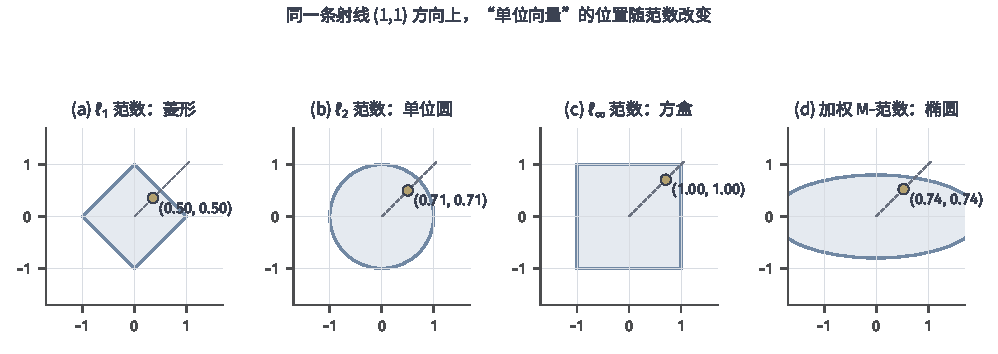
\includegraphics[width=169mm]{figures/00-shared/mathematical-preliminaries-upper/02-linear-spaces/matplotlib/ls-norm-unit-balls/ls-norm-unit-balls.pdf}
  \caption{同一向量在不同范数下的“单位球”形状。左：$\ell_1$单位球为菱形（累加绝对偏差）；中：$\ell_2$单位球为圆（欧氏长度）；右：$\ell_\infty$单位球为正方形（最大坐标偏差）。同一个点$(1,1)$的范数依次为$2$、$\sqrt2$、$1$，单位球大小随口径而变，三者之间的倍数关系将在第~\ref{sec:ls-norms-distances}节给出。三图坐标尺度相同，为解析教学例。}
  \label{fig:ls-norm-unit-balls}
\end{figure*}

本节建立了坐标向量的基本计算：加法、数乘与线性组合产生新的向量，欧氏内积把两个向量配成一个数，常用范数度量向量的大小。加法与数乘的规则将用于定义线性空间；内积与范数的一般性质留到第~\ref{chap:normed-inner-product-spaces}章。把若干向量并排放在一起，就得到下一节的矩阵。
